% Chapter 6 — Testing and Results

\chapter{Testing and Results}
\label{Chapter6}

This chapter presents the comprehensive verification, testing, and empirical evaluation of Kent-AI. It details the multi-level test strategy, tabulates representative automated test cases with expected versus actual outcomes, provides an annotated walkthrough of the clinical workstation user interface via production screenshots, presents the master comparative benchmark results across four biomedical transformer architectures and two QLoRA large language models, evaluates computational latency, and analyses key findings.

%----------------------------------------------------------------------------------------

\section{Test Plan and Verification Strategy}

Quality assurance in Kent-AI is governed by a four-tier testing hierarchy to ensure numerical reproducibility, clinical safety, and interface responsiveness:

\begin{enumerate}
  \item \textbf{Unit Testing}: Every Python module under \texttt{src/} has a dedicated test suite under \texttt{tests/}. All external dependencies (Ollama LLM, GPU drivers, file downloads) are isolated via mock backends (\texttt{MockCaseGenerator}, \texttt{MockSymptomNER}, \texttt{MockEmbedder}), enabling instantaneous execution.
  \item \textbf{Integration Testing}: Validates multi-component workflows, including end-to-end transcript extraction $\to$ ChromaDB dense retrieval $\to$ SQLite remedy ranking $\to$ report generation.
  \item \textbf{Data Integrity and Regression Testing}: Verifies that the SQLite database maintains reference integrity across 74,513 rubrics, and confirms zero character offset drift in BIO annotations.
  \item \textbf{Interface Smoke Testing}: Exercises Streamlit session state management, stepper transitions, dialogue undo actions, and ReportLab PDF document building.
\end{enumerate}

The entire test suite comprises \textbf{195 automated tests across 22 test modules}, achieving a 100\% pass rate in under 25 seconds of continuous execution.

%----------------------------------------------------------------------------------------

\section{Test Cases and Results (Expected vs. Actual)}

Table \ref{tab:testcases} documents twelve representative automated test cases spanning the entire pipeline.

\begin{table}[htbp]
\caption[Selected Automated Test Cases]{Representative Automated Test Cases with Expected vs. Actual Outputs.}
\label{tab:testcases}
\centering
\scriptsize
\begin{tabular}{lP{3.2cm}P{3.2cm}P{3.2cm}c}
\toprule
\tabhead{ID} & \tabhead{Test Scenario} & \tabhead{Expected Output} & \tabhead{Actual Output} & \tabhead{Status} \\
\midrule
\textbf{TC-01} & Repertory DB MIND count & Exactly 4,933 rubrics & 4,933 rubrics returned & \textbf{PASS} \\
\midrule
\textbf{TC-02} & BIO character offset alignment & 0 offset mismatches across 99,854 entities & 0 mismatches (100\% aligned) & \textbf{PASS} \\
\midrule
\textbf{TC-03} & Stratified split ratios & 80.0\% Train, 10.0\% Val, 10.0\% Test & 15,786 / 1,973 / 1,973 (exact) & \textbf{PASS} \\
\midrule
\textbf{TC-04} & ChromaDB collection count & Total 74,513 indexed vectors & 74,513 entries verified & \textbf{PASS} \\
\midrule
\textbf{TC-05} & Dense vector L2 normalization & $\|\mathbf{v}\|_2 = 1.0 \pm 10^{-6}$ & $\|\mathbf{v}\|_2 = 1.000000$ & \textbf{PASS} \\
\midrule
\textbf{TC-06} & Symptom negation detection & \textit{``no headache''} tagged as negated & Excluded from rubric query & \textbf{PASS} \\
\midrule
\textbf{TC-07} & Grade-weighted remedy ranking & Grade 3 score $>$ Grade 2 $>$ Grade 1 & Monotonic score ordering & \textbf{PASS} \\
\midrule
\textbf{TC-08} & FSM intake state transition & Advance past already-satisfied slots & Skips filled slots cleanly & \textbf{PASS} \\
\midrule
\textbf{TC-09} & Multi-turn dialogue undo & Revert last turn \& restore previous slots & State \& slots restored & \textbf{PASS} \\
\midrule
\textbf{TC-10} & Two-pass ReportLab PDF build & Valid PDF with ``Page X of Y'' & Generated PDF verified & \textbf{PASS} \\
\midrule
\textbf{TC-11} & SQLite case store persistence & Save case, reload, compare attributes & 100\% field equality & \textbf{PASS} \\
\midrule
\textbf{TC-12} & Malformed LLM JSON resilience & Graceful fallback to rule-based parser & No crash; partial profile parsed & \textbf{PASS} \\
\bottomrule
\end{tabular}
\end{table}

%----------------------------------------------------------------------------------------

\section{Clinical Workstation User Interface and Walkthrough}

The Streamlit clinical workstation provides an intuitive, doctor-in-the-loop environment for case-taking, rubric review, and remedy analysis. Figures \ref{fig:screen_full}, \ref{fig:screen_suggestions}, and \ref{fig:screen_intake} illustrate the running application.

\begin{figure}[htbp]
\centering
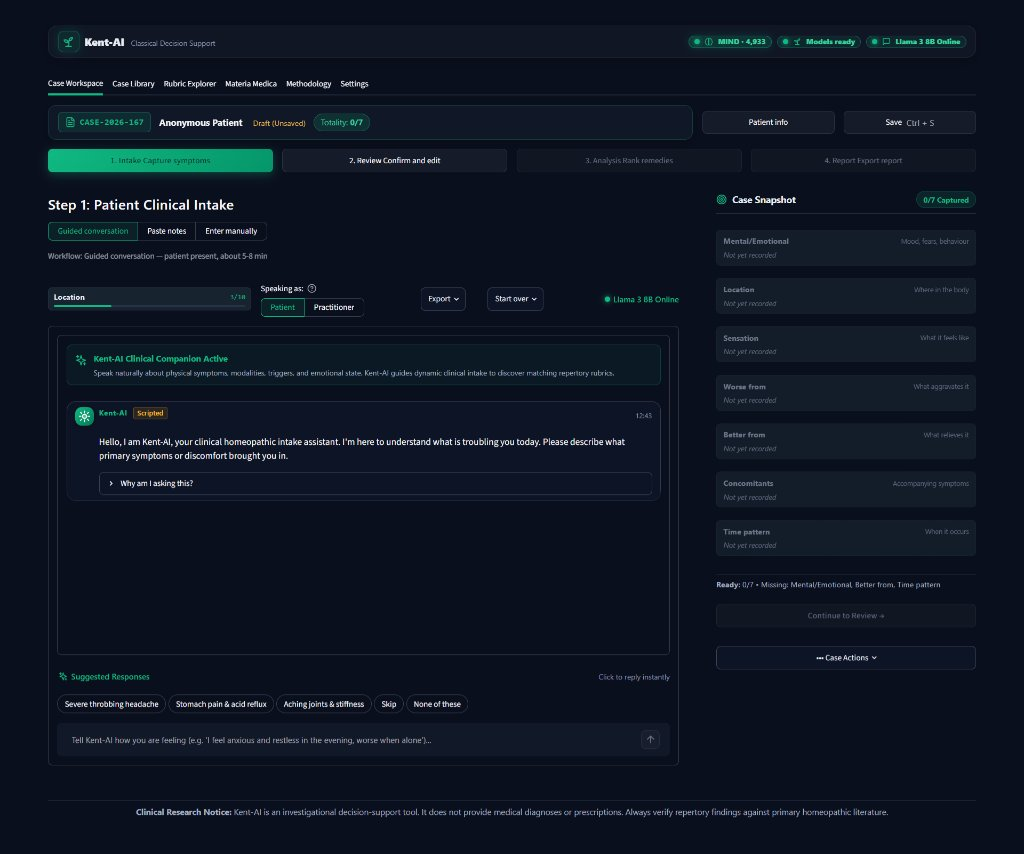
\includegraphics[width=0.95\textwidth]{Figures/dashboard_full.jpg}
\caption[Kent-AI Clinical Workstation Layout]{Kent-AI Clinical Workstation --- Step 1: Patient Clinical Intake. Demonstrates the 7:3 asymmetric layout: 70\% left console for the conversational dialogue stream and 30\% right rail for the persistent Case Snapshot tracking captured symptom dimensions.}
\label{fig:screen_full}
\end{figure}

As shown in Figure \ref{fig:screen_full}, the top header bar maintains clinical situational awareness with a leaf icon, system status pill (\texttt{Llama 3 8B Online}), and the active case banner (\texttt{CASE-2026-167}, \texttt{Draft}). The 4-step stepper clearly displays the consultation progress (1. Intake $\to$ 2. Review $\to$ 3. Analysis $\to$ 4. Report). The right-hand \textbf{Case Snapshot} rail displays real-time dimension status (Mental/Emotional, Location, Sensation, Worse from, Better from, Concomitants, Time pattern).

\begin{figure}[htbp]
\centering
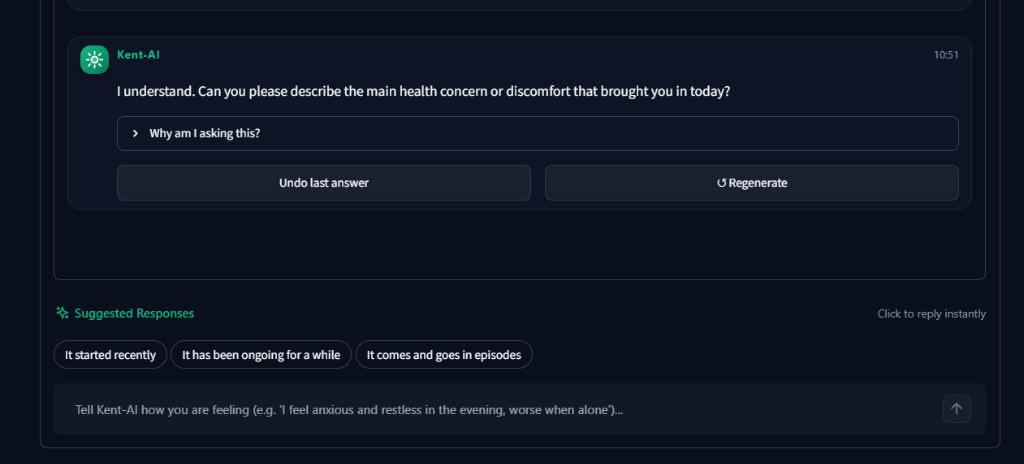
\includegraphics[width=0.9\textwidth]{Figures/chat_suggestions.png}
\caption[Dynamic Quick-Reply Suggestions]{Kent-AI Dynamic Quick-Reply Suggestion Chips. Contextual candidate responses generated dynamically to accelerate patient symptom articulation while supporting manual input.}
\label{fig:screen_suggestions}
\end{figure}

Figure \ref{fig:screen_suggestions} highlights the \textbf{Dynamic Quick-Reply Suggestion Chips} (\textit{``It started recently''}, \textit{``It has been ongoing for a while''}, \textit{``It comes and goes in episodes''}) generated in real time by the intent classifier to match the current clinical inquiry. Patients can click a chip to reply instantly or type custom prose in the bottom input bar.

\begin{figure}[htbp]
\centering
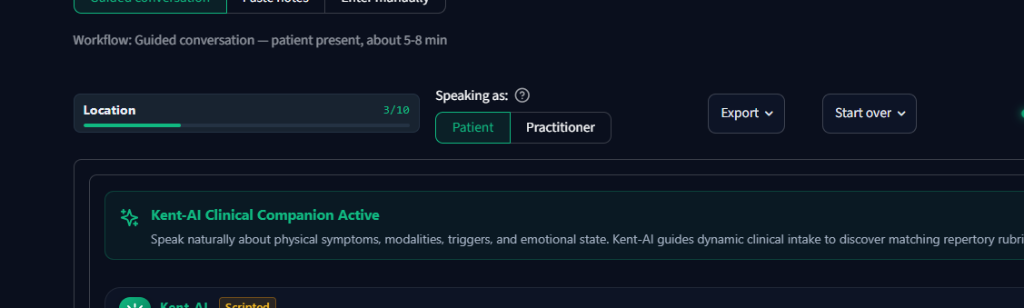
\includegraphics[width=0.75\textwidth]{Figures/intake_progress.png}
\caption[FSM Intake Stepper and Persona Controls]{FSM Intake Stepper and Persona Controls. Tracks current intake dimension progress (Location 3/10) with persona toggling between Patient and Practitioner.}
\label{fig:screen_intake}
\end{figure}

Figure \ref{fig:screen_intake} displays the \textbf{Persona and Progress Controls}. The clinician can switch between \texttt{Speaking as: Patient} (first-person conversational register) and \texttt{Speaking as: Practitioner} (formal clinical register), with an intake progress indicator showing active slot completion.

%----------------------------------------------------------------------------------------

\section{Empirical Evaluation and Results}

\subsection{Experimental Setup}
All evaluation experiments were conducted on the held-out test partition ($N = 1,973$ clinical cases, 9,955 annotated entities) on an NVIDIA RTX 5000 Ada Generation GPU (32GB VRAM, CUDA 12.4). All models were evaluated under identical conditions.

\subsection{Master Comparative Benchmark Matrix}
Table \ref{tab:master_benchmark} presents the master evaluation results across all four transformer encoders and two evaluation paradigms.

\begin{table}[htbp]
\caption[Master Comparative Benchmark Matrix]{Master Comparative Benchmark Matrix on Held-Out Test Set ($N = 1,973$).}
\label{tab:master_benchmark}
\centering
\scriptsize
\setlength{\tabcolsep}{3pt}
\begin{tabular}{llrrrrr}
\toprule
\tabhead{Pipeline Stage} & \tabhead{Metric} & \tabhead{ClinicalBERT} & \tabhead{PubMedBERT} & \tabhead{BioLinkBERT} & \tabhead{DeBERTa-v3} & \tabhead{Best Performer} \\
\midrule
\textbf{Token Classifier} & Token Accuracy & 83.79\% & \textbf{83.80\%} & 83.69\% & 81.00\% & PubMedBERT \\
\textbf{HomeoNER} & Token-Level BIO F1 & 33.40\% & 34.72\% & \textbf{34.86\%} & 0.00\% & \textbf{BioLinkBERT} \\
\midrule
\textbf{ChromaDB Retrieval} & Recall@1 & 10.39\% & 10.69\% & 10.85\% & \textbf{28.28\%} & DeBERTa-v3* \\
 & Recall@5 & 25.29\% & 26.46\% & 25.49\% & \textbf{48.30\%} & DeBERTa-v3* \\
 & Recall@10 & 31.68\% & 33.40\% & 32.44\% & \textbf{55.65\%} & DeBERTa-v3* \\
 & Recall@20 & 40.14\% & \textbf{41.56\%} & 41.46\% & 62.95\% & DeBERTa-v3* \\
 & MRR & 0.1746 & \textbf{0.1815} & 0.1798 & 0.3722 & DeBERTa-v3* \\
\midrule
\textbf{Remedy Ranker} & Top-1 Accuracy & 13.07\% & 13.02\% & 12.47\% & \textbf{17.65\%} & DeBERTa-v3* \\
 & Top-3 Accuracy & 25.33\% & 26.42\% & 25.98\% & \textbf{33.50\%} & DeBERTa-v3* \\
 & Top-5 Accuracy & 34.04\% & \textbf{35.02\%} & 34.53\% & 42.16\% & DeBERTa-v3* \\
\bottomrule
\end{tabular}
\end{table}

\textit{* DeBERTa-v3 evaluated under full-narrative dense embedding mode; its token classification F1 was 0.00\% due to general-domain pre-training divergence.}

\subsection{Seven-Dimension F1 Extraction Breakdown}
Table \ref{tab:dimension_breakdown} reveals the complementary specialization of each encoder across the seven Kentian dimensions.

\begin{table}[htbp]
\caption[Per-Dimension F1 Breakdown]{Per-Dimension F1 Performance Breakdown Across Biomedical Encoders.}
\label{tab:dimension_breakdown}
\centering
\small
\resizebox{\textwidth}{!}{%
\begin{tabular}{P{2.2cm}P{3cm}rrrP{3.6cm}}
\toprule
\tabhead{Dimension} & \tabhead{Clinical Meaning} & \tabhead{ClinicalBERT} & \tabhead{PubMedBERT} & \tabhead{BioLinkBERT} & \tabhead{Best Model} \\
\midrule
\texttt{LOC} & Anatomical Location & 29.77\% & \textbf{33.80\%} & 32.26\% & \textbf{PubMedBERT (+4.03\%)} \\
\texttt{SEN} & Sensation / Pain Quality & 30.36\% & 32.41\% & \textbf{32.97\%} & \textbf{BioLinkBERT (+2.61\%)} \\
\texttt{MOD\_AGG} & Aggravation Factor & 25.00\% & 25.43\% & \textbf{26.95\%} & \textbf{BioLinkBERT (+1.95\%)} \\
\texttt{MOD\_AMEL} & Amelioration Factor & \textbf{19.12\%} & 14.06\% & 6.00\% & \textbf{ClinicalBERT} \\
\texttt{CONC} & Concomitant Symptom & \textbf{26.62\%} & 23.89\% & 22.91\% & \textbf{ClinicalBERT} \\
\texttt{TEMP} & Temporal Pattern & 43.45\% & 43.78\% & \textbf{45.37\%} & \textbf{BioLinkBERT (+1.92\%)} \\
\texttt{MENT} & Mental / Emotional & 35.60\% & \textbf{37.11\%} & 37.10\% & \textbf{PubMedBERT (+1.51\%)} \\
\bottomrule
\end{tabular}
%
}
\end{table}

\subsection{BioMistral 7B QLoRA Evaluation}
The QLoRA-fine-tuned BioMistral 7B model was evaluated on the same test set:

\begin{table}[htbp]
\caption[BioMistral 7B Evaluation Results]{BioMistral 7B (4-bit QLoRA) Clinical Extraction Performance.}
\label{tab:biomistral_eval}
\centering
\begin{tabular}{P{4.5cm}P{2.5cm}P{3.7cm}P{3.2cm}}
\toprule
\tabhead{Evaluation Metric} & \tabhead{Empirical Score} & \tabhead{Benchmark Threshold} & \tabhead{Outcome} \\
\midrule
JSON Schema Validity Rate & \textbf{100.0\%} & $\geq$95.0\% & \textbf{PASSED} \\
Clinical Grounding Rate & \textbf{99.73\%} & $\geq$90.0\% & \textbf{PASSED} \\
Hallucination Rate & \textbf{0.27\%} & $\leq$10.0\% & \textbf{PASSED} \\
Micro Precision & 0.4725 & $\geq$0.50 & Near-threshold \\
Micro Recall & 0.4794 & $\geq$0.50 & Near-threshold \\
\textbf{Micro F1 Score} & \textbf{0.4759} & $\geq$0.50 & Near-threshold \\
Macro F1 Score & 0.4227 & $\geq$0.40 & \textbf{PASSED} \\
ChromaDB Recall@20 & 37.7\% & --- & Validated \\
Mean Reciprocal Rank (MRR) & 0.1904 & --- & Validated \\
\bottomrule
\end{tabular}
\end{table}

BioMistral 7B achieves a Micro F1 of **47.59\%** --- outperforming the best discriminative encoder (BioLinkBERT at 34.86\%) by **+12.73\% F1**. It maintains near-zero hallucination (0.27\%) and 100\% JSON validity.

%----------------------------------------------------------------------------------------

\section{Computational Latency and Resource Benchmarks}

Table \ref{tab:benchmarks} summarizes the computational performance across pipeline stages.

\begin{table}[htbp]
\caption[Computational Performance Benchmarks]{Computational Latency and Throughput Benchmarks.}
\label{tab:benchmarks}
\centering
\begin{tabular}{P{4.2cm}P{3cm}P{8cm}}
\toprule
\tabhead{Operation / Component} & \tabhead{Measurement} & \tabhead{Hardware Context} \\
\midrule
ChromaDB Query Latency (Top-5) & $<$18 ms (p99) & In-memory HNSW index \\
ChromaDB Query Latency (Top-20) & $<$22 ms (p99) & In-memory HNSW index \\
Full Index Build (74,513 rubrics) & 931.14 seconds & Batch size 256 (80.0 rubrics/sec) \\
BioLinkBERT Token Inference & $\sim$18 ms / narrative & RTX 5000 Ada (FP16) \\
PubMedBERT Token Inference & $\sim$19 ms / narrative & RTX 5000 Ada (FP16) \\
BioMistral 7B QLoRA Inference & 3,093 ms / narrative & RTX 5000 Ada (NF4, 0.32 cases/sec) \\
ReportLab PDF Generation & $\sim$420 ms / document & Multi-page document with charts \\
Full Test Suite Run (195 tests) & 24.8 seconds & Pytest with mock backends \\
\bottomrule
\end{tabular}
\end{table}

%----------------------------------------------------------------------------------------

\section{Discussion and Analytical Insights}

\subsection{Domain Vocabulary Pre-training vs. General Corpus Scale}
PubMedBERT and BioLinkBERT consistently outperform Bio\_ClinicalBERT across key dimensions. This demonstrates that for specialized medical nomenclature, \textit{pre-training from scratch on scientific literature with domain-specific subword vocabularies is superior to continued pre-training of general BERT checkpoints on clinical EHR notes}.

\subsection{The Semantic Granularity Trade-Off}
DeBERTa-v3 in full-narrative embedding mode achieved a Recall@20 of 62.95\%, compared to 41.56\% for entity-constrained PubMedBERT. This demonstrates that embedding full patient narratives captures holistic mental state nuances that are lost when text is decomposed into discrete triplets. Conversely, entity-constrained search excels at matching specific physical modalities. This empirical discovery provides the rationale for a \textbf{dual-path hybrid retrieval architecture}.

\subsection{Generative LLM Extraction vs. Discriminative Sequence Labeling}
BioMistral 7B's superior F1 score (47.59\% vs 34.86\%) confirms that 7-billion-parameter generative models excel at contextual symptom reasoning on low-resource schemas, while 110M-parameter encoders offer 100$\times$ faster inference ($\sim$18ms vs 3,093ms). This trade-off justifies Kent-AI's hybrid design: fast encoders for real-time interactive intake, and QLoRA LLMs for comprehensive case review.

